\chapter{System Architecture}
\label{chap:arch}

This chapter presents information concerning the architecture of the software
system both from the static and dynamic viewpoints. The static viewpoint focuses
on the physical architecture (hardware) required to deploy and run the
software system along with the manner in which the components that make such
software system are grouped. On the other hand, the dynamic viewpoint focuses on
the behaviour of the software system at runtime. 

The static information is presented through the \gls{Deployment View} and the
\gls{Implementation View}. The dynamic aspects of the system are presented by
means of the \gls{UI Processing View}.


\section{Deployment view}
System's architecture follows client-server software architecture with 3 layers.

\begin{figure}
\begin{center}
\includegraphics[width=0.7\textwidth]{./images/Architecture.eps}
\end{center}
\caption{Deployment view}
\end{figure}

\begin{itemize}
  \item Client's layer holds the UIs
  \item Server's layer holds the system operations
  \item Database's layer holds the data persistance
\end{itemize}

\begin{center}
\textbf{iCrash desktop application deployment view}
\end{center}

\begin{figure}[H]
\begin{center}
\includegraphics[width=0.9\textwidth]{./images/depl_model.eps}
\end{center}
\caption{iCrash desktop application deployment view}
\end{figure}

\begin{center}
\textbf{iCrash web application deployment view}
\end{center}

\begin{figure}[H]
\begin{center}
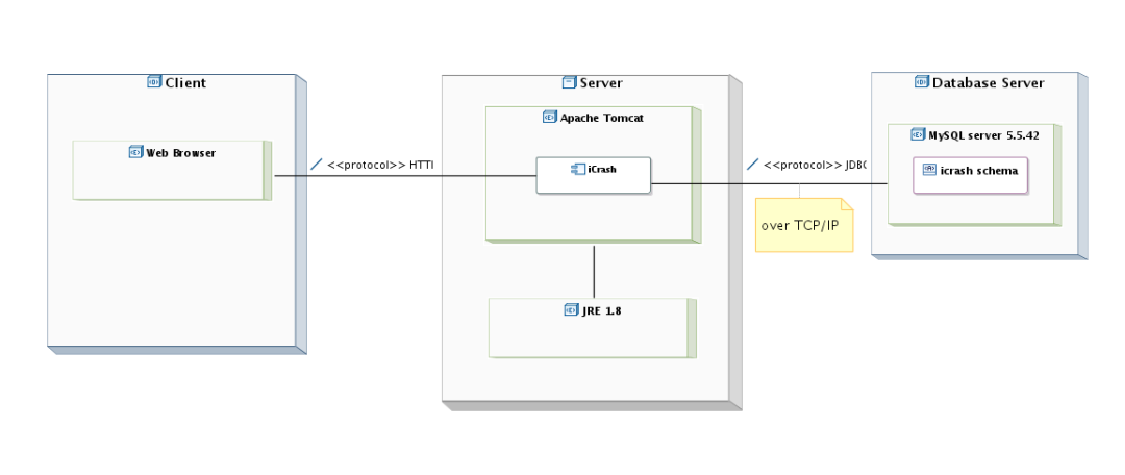
\includegraphics[width=0.9\textwidth]{./images/depl_model_web.eps}
\end{center}
\caption{iCrash web application deployment view}
\end{figure}

\section{Implementation view}
The \gls{Implementation View} describes each software system component and how
they are organised and combined to make the targeted software system.



\begin{figure}[h!]
	\centering
	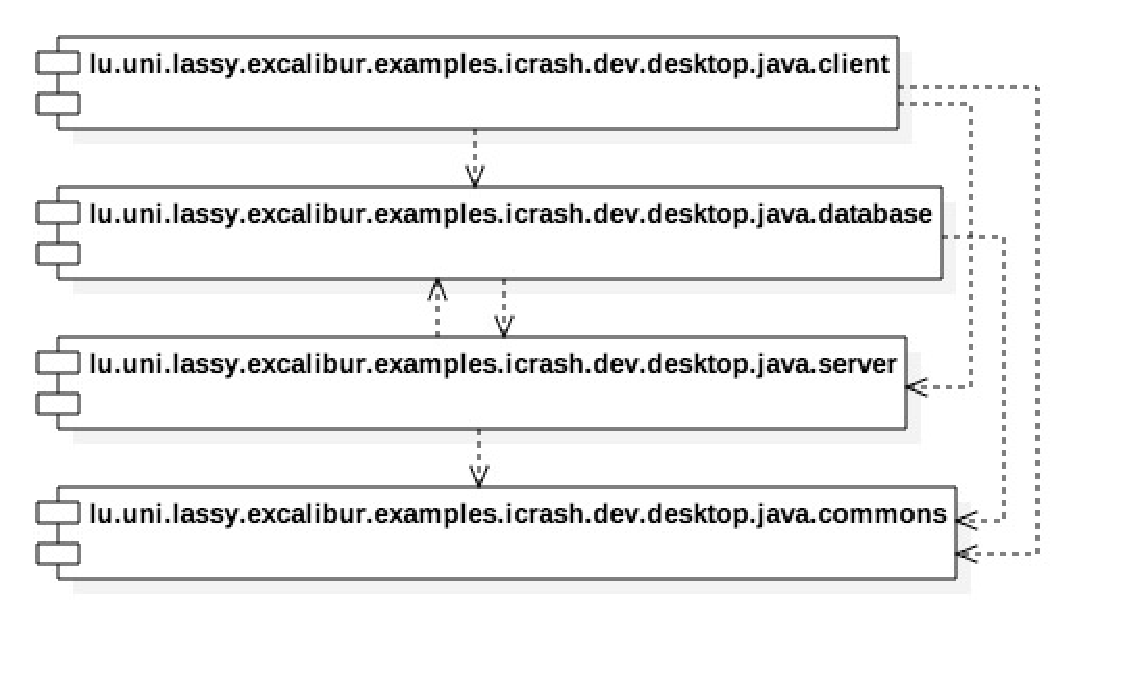
\includegraphics[width=0.9\textwidth]{./images/impl_highlevel.eps}
	\caption{Implementation View - High level}
\end{figure}

\begin{figure}[h!]
	\centering
	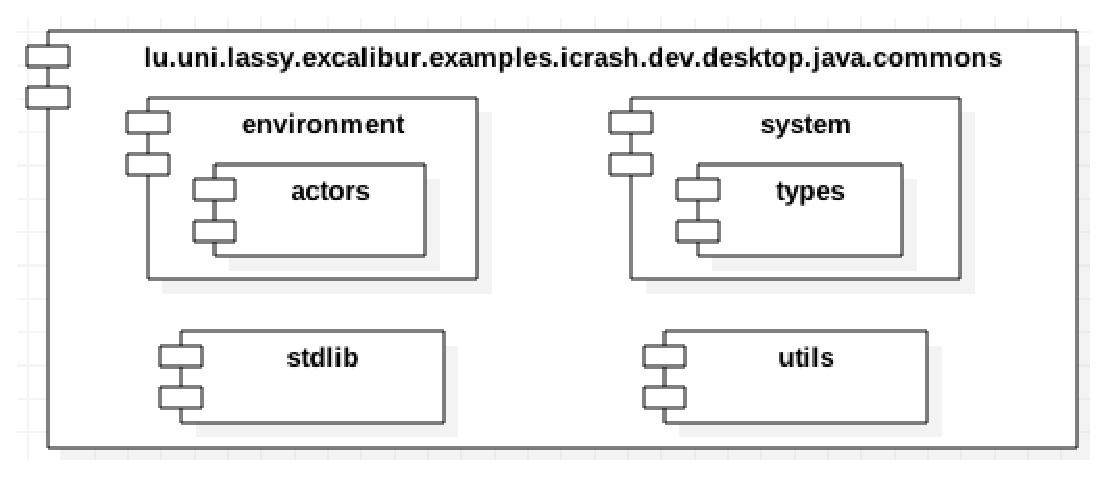
\includegraphics[width=0.9\textwidth]{./images/impl_commons.eps}
	\caption{Implementation View - Commons component}
\end{figure}

\begin{figure}[h!]
	\centering
	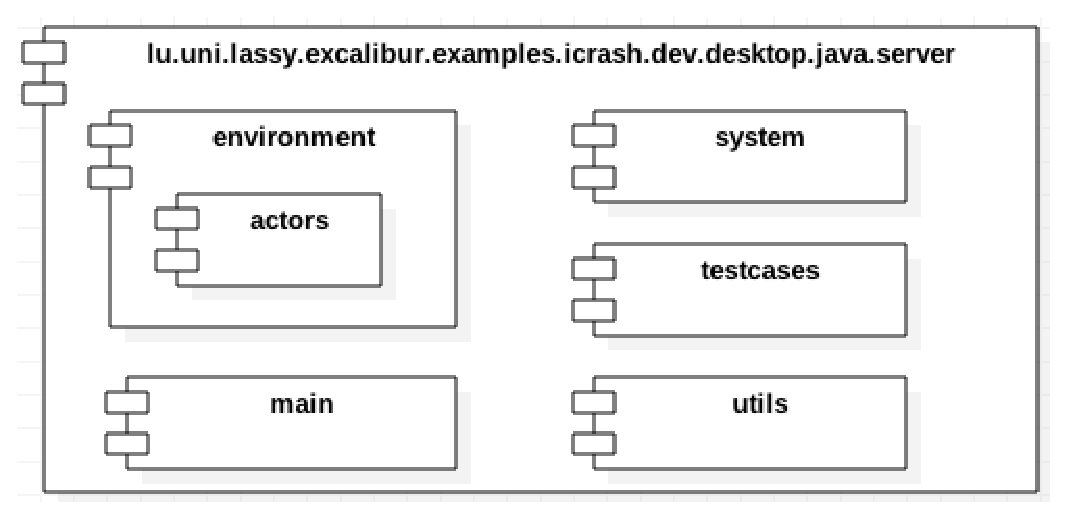
\includegraphics[width=0.9\textwidth]{./images/impl_server.eps}
	\caption{Implementation View - Server component}
\end{figure}

\begin{figure}[h!]
	\centering
	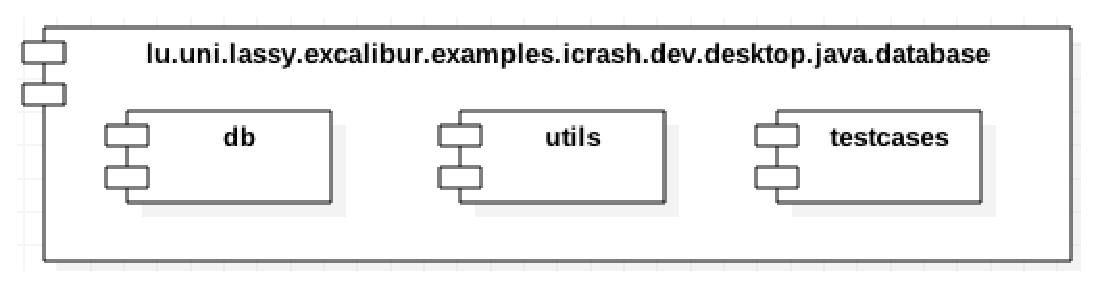
\includegraphics[width=0.9\textwidth]{./images/impl_db.eps}
	\caption{Implementation View - Database component}
\end{figure}

\begin{figure}[h!]
	\centering
	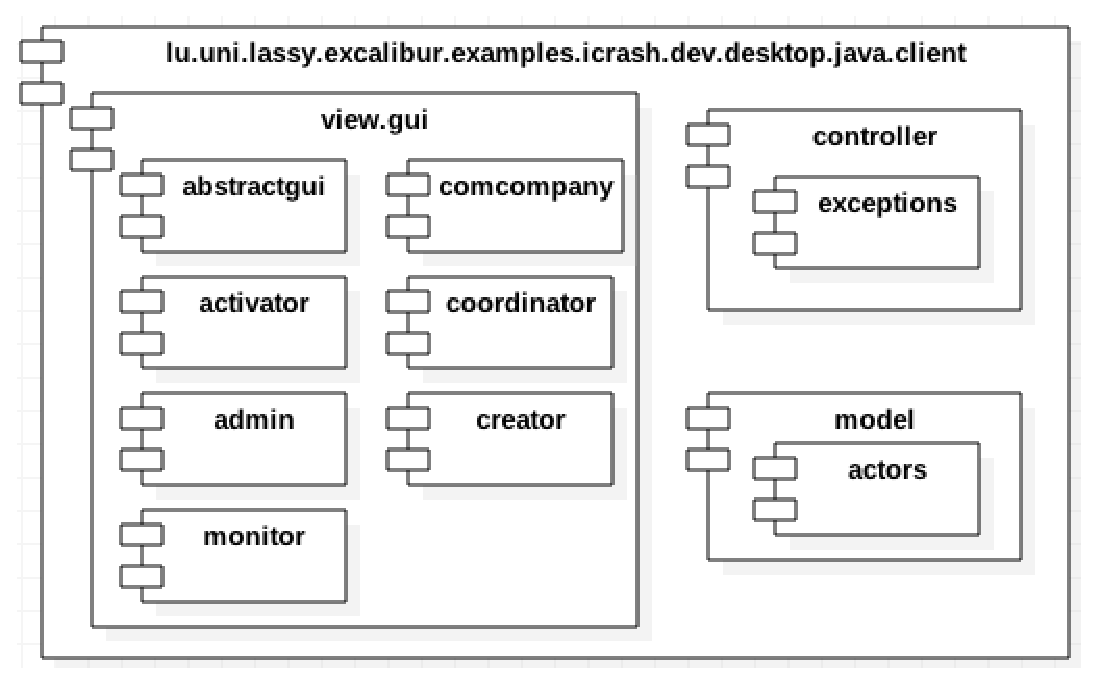
\includegraphics[width=0.9\textwidth]{./images/impl_client.eps}
	\caption{Implementation View - Client component}
\end{figure}





\section{UI Processing view}
A \gls{UI Processing View} is aimed at explaining the required message
exchanges to achieve the launching of a system operation (specified in the \msrmessir
Analysis Document). 
%These required message exchanges (which are not specified
% in the \msrmessir Analysis Document) make part of the user interface (UI). Thus, the
%main interest of a UI Processing View is to describe the design choices made
%at the UI level, such that a system operation is launched. The description
%of a UI Processing View is given by means of a UML Sequence Diagram. 


%A complete Design Document should contain a UI Processing View for each
%non-proactive system operation specified in the \msrmessir Analysis Document,
% as such kind of system operations are launched by actors through UIs that allows
%them to make so. 



\subsection{UI Processing view for system operation oeAddCoordinator}
\begin{figure}[h]
	\centering	
	\captionsetup{justification=centering}
	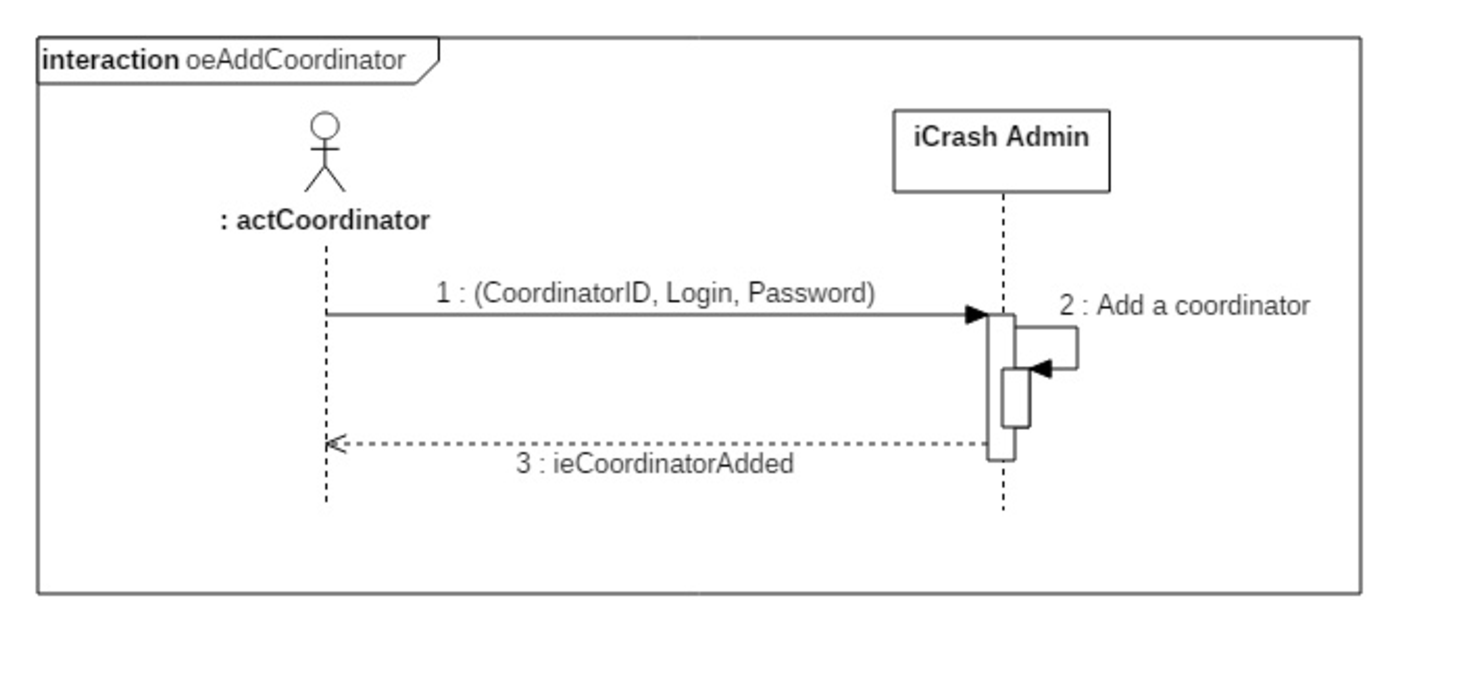
\includegraphics[width=0.5\textwidth]{./images/ui_oeAddCoordinator.eps}
	\caption{UI Processing view - oeAddCoordinator}
\end{figure}
 
\subsection{UI Processing view for system operation oeAlert}

\begin{figure}[h]
	\centering	
	\captionsetup{justification=centering}
	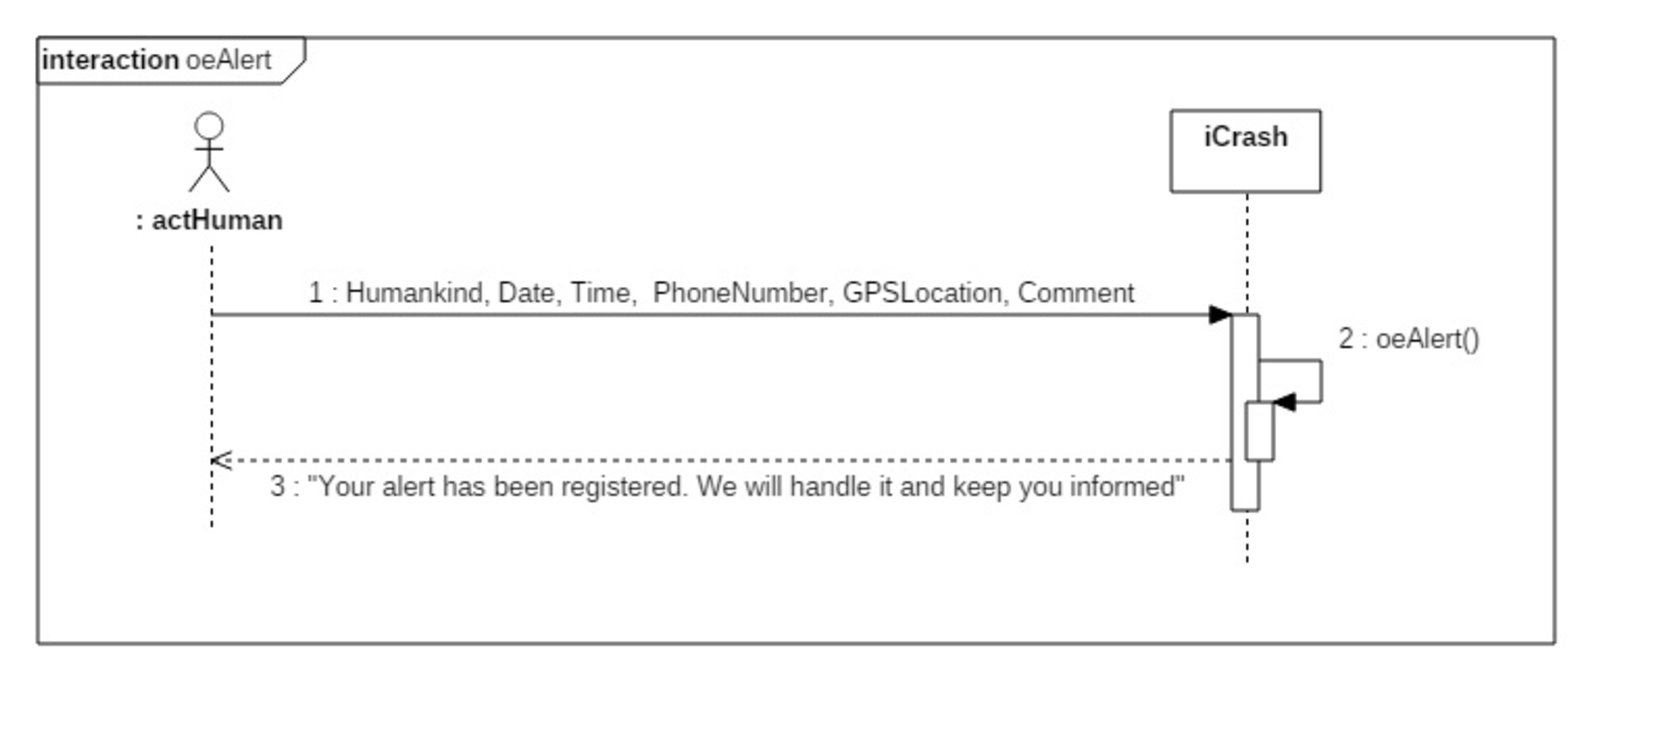
\includegraphics[width=0.75\textwidth]{./images/ui_oeAlert.eps}
	\caption{UI Processing view - oeAlert}
\end{figure}


\subsection{UI Processing view for system operation oeCloseCrisis}

\begin{figure}[h]
	\centering	
	\captionsetup{justification=centering}
	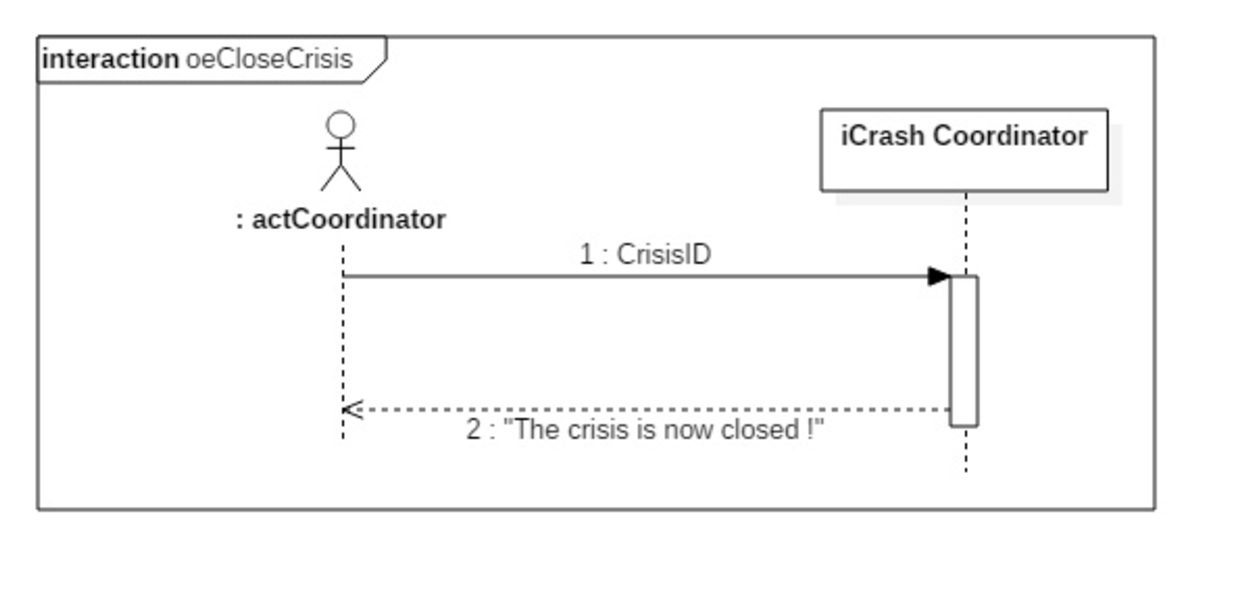
\includegraphics[width=0.5\textwidth]{./images/ui_oeCloseCrisis.eps}
	\caption{UI Processing view - oeCloseCrisis}
\end{figure}


\subsection{UI Processing view for system operation oeDeleteCoordinator}

\begin{figure}[h]
	\centering	
	\captionsetup{justification=centering}
	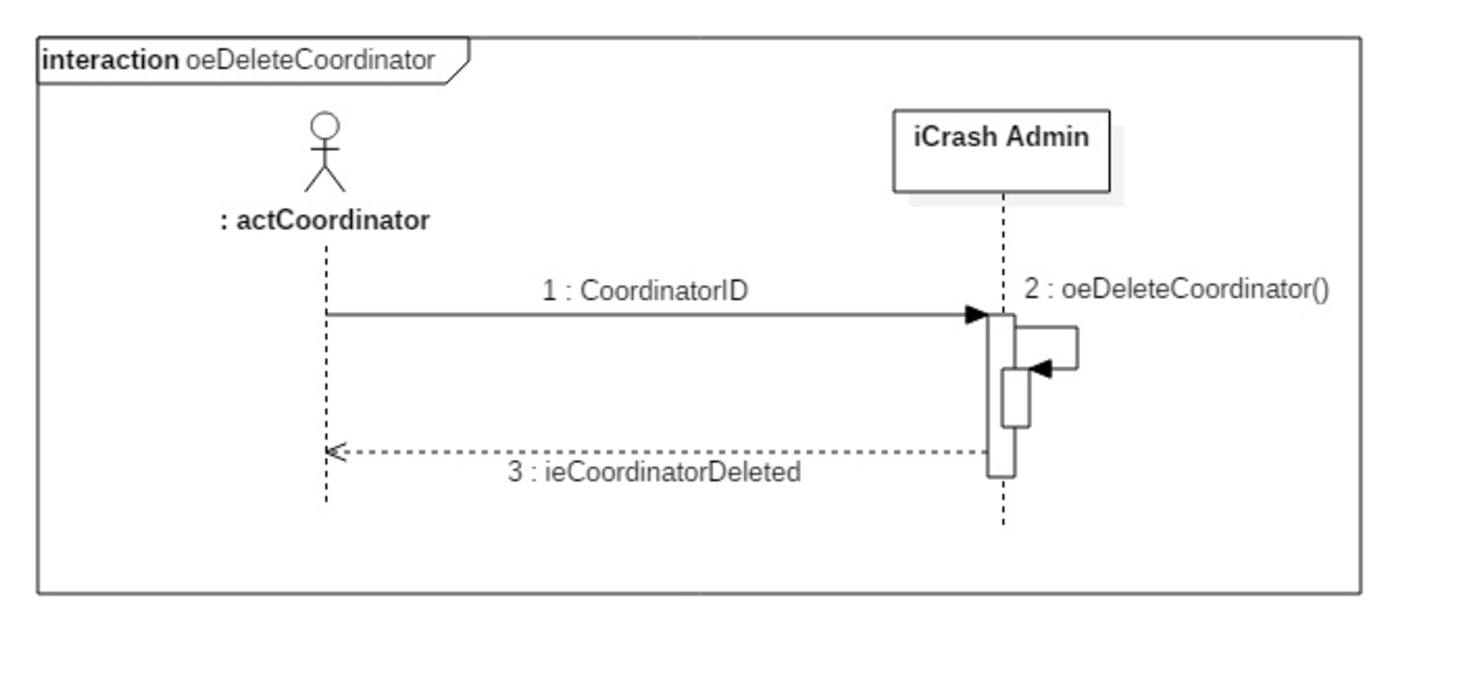
\includegraphics[width=0.5\textwidth]{./images/ui_oeDeleteCoordinator.eps}
	\caption{UI Processing view - oeDeleteCoordinator}
\end{figure}


\subsection{UI Processing view for system operation oeInvalidateAlert}

\begin{figure}[h]
	\centering	
	\captionsetup{justification=centering}
	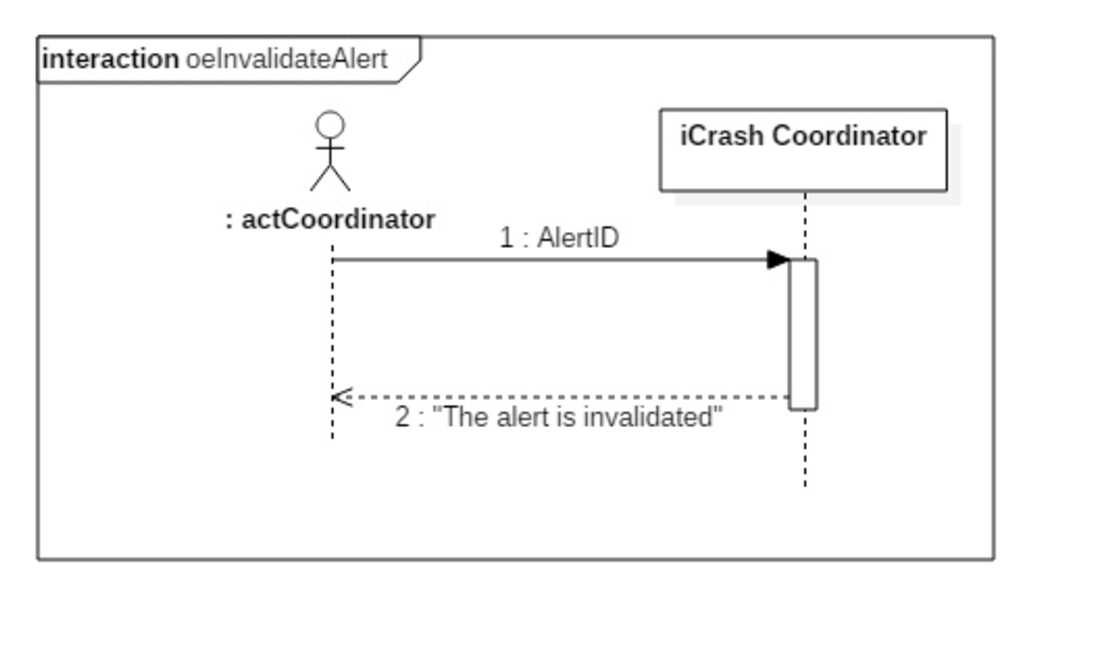
\includegraphics[width=0.5\textwidth]{./images/ui_oeInvalidateAlert.eps}
	\caption{UI Processing view - oeInvalidateAlert}
\end{figure}


\subsection{UI Processing view for system operation oeLogin}

\begin{figure}[h]
	\centering	
	\captionsetup{justification=centering}
	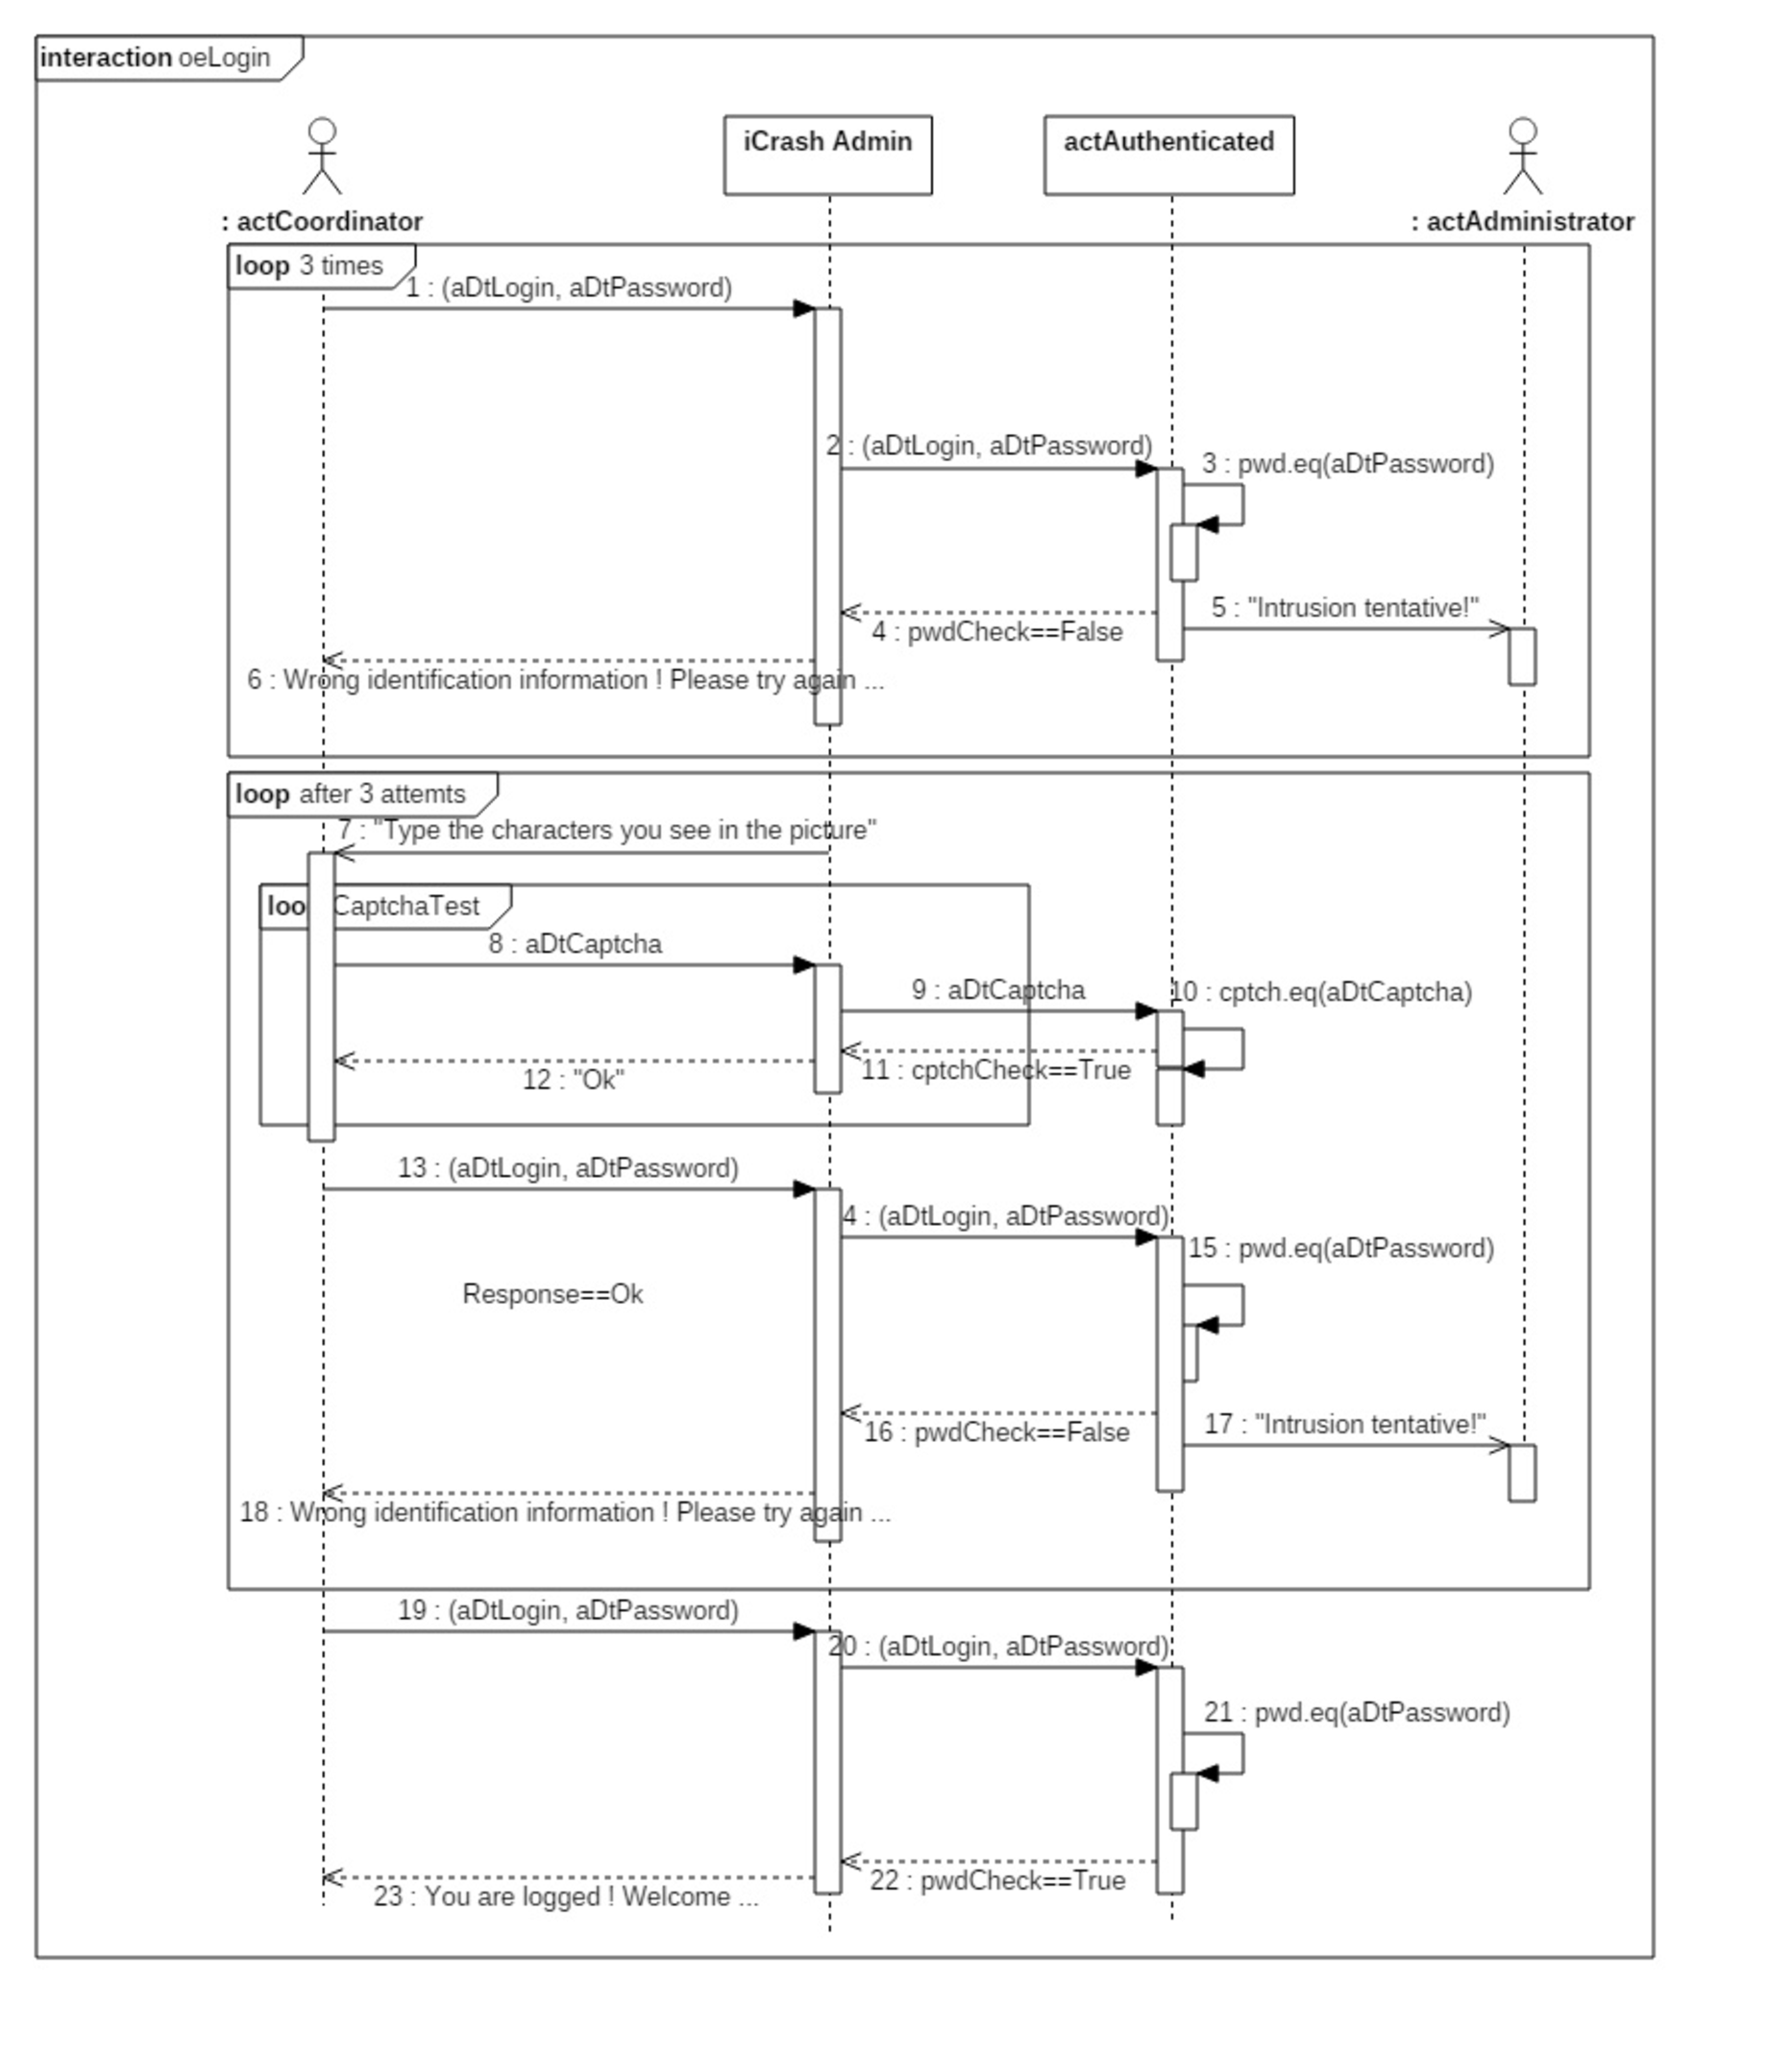
\includegraphics[width=0.75\textwidth]{./images/ui_oeLogin.eps}
	\caption{UI Processing view - oeLogin}
\end{figure}


\subsection{UI Processing view for system operation oeLogout}

\begin{figure}[h]
	\centering	
	\captionsetup{justification=centering}
	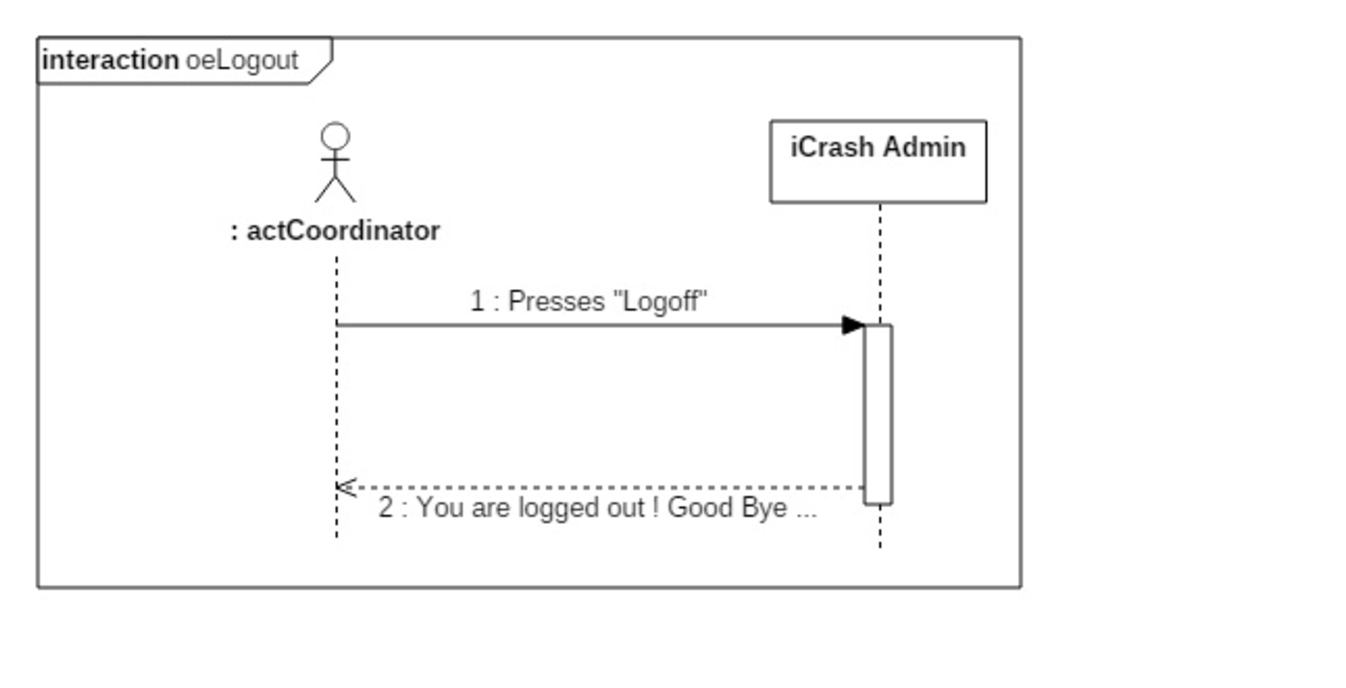
\includegraphics[width=0.5\textwidth]{./images/ui_oeLogout.eps}
	\caption{UI Processing view - oeLogout}
\end{figure}


\subsection{UI Processing view for system operation oeReportOnCrisis}

\begin{figure}[h]
	\centering	
	\captionsetup{justification=centering}
	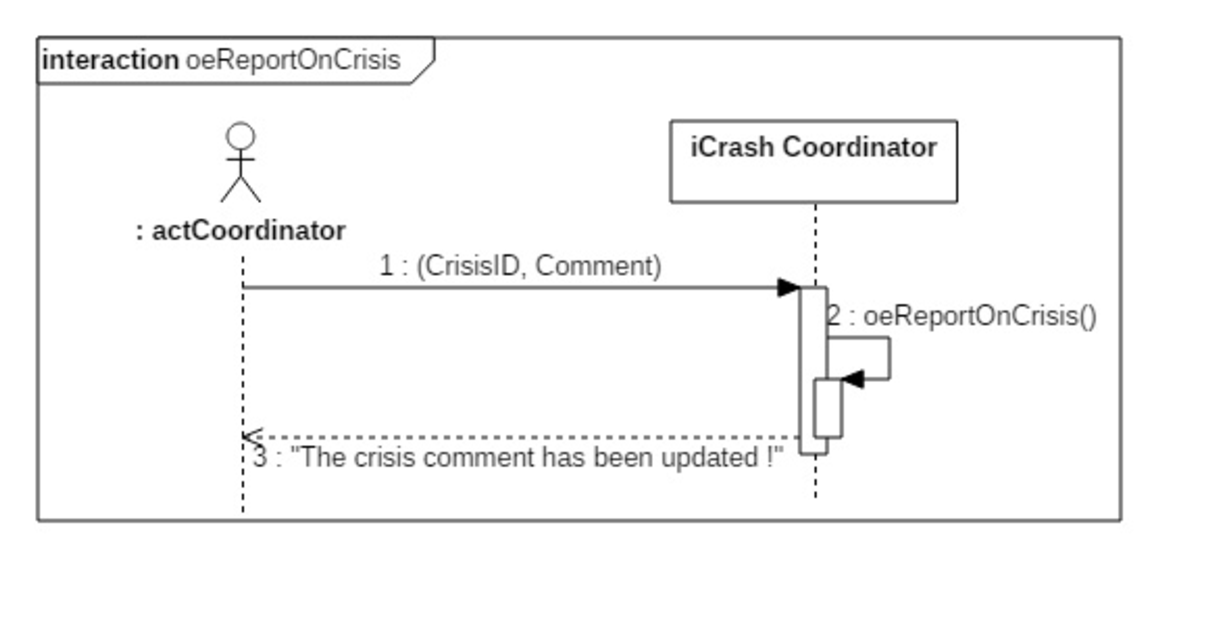
\includegraphics[width=0.5\textwidth]{./images/ui_oeReportOnCrisis.eps}
	\caption{UI Processing view - oeReportOnCrisis}
\end{figure}


\subsection{UI Processing view for system operation oeSetCrisisHandler}

\begin{figure}[h]
	\centering	
	\captionsetup{justification=centering}
	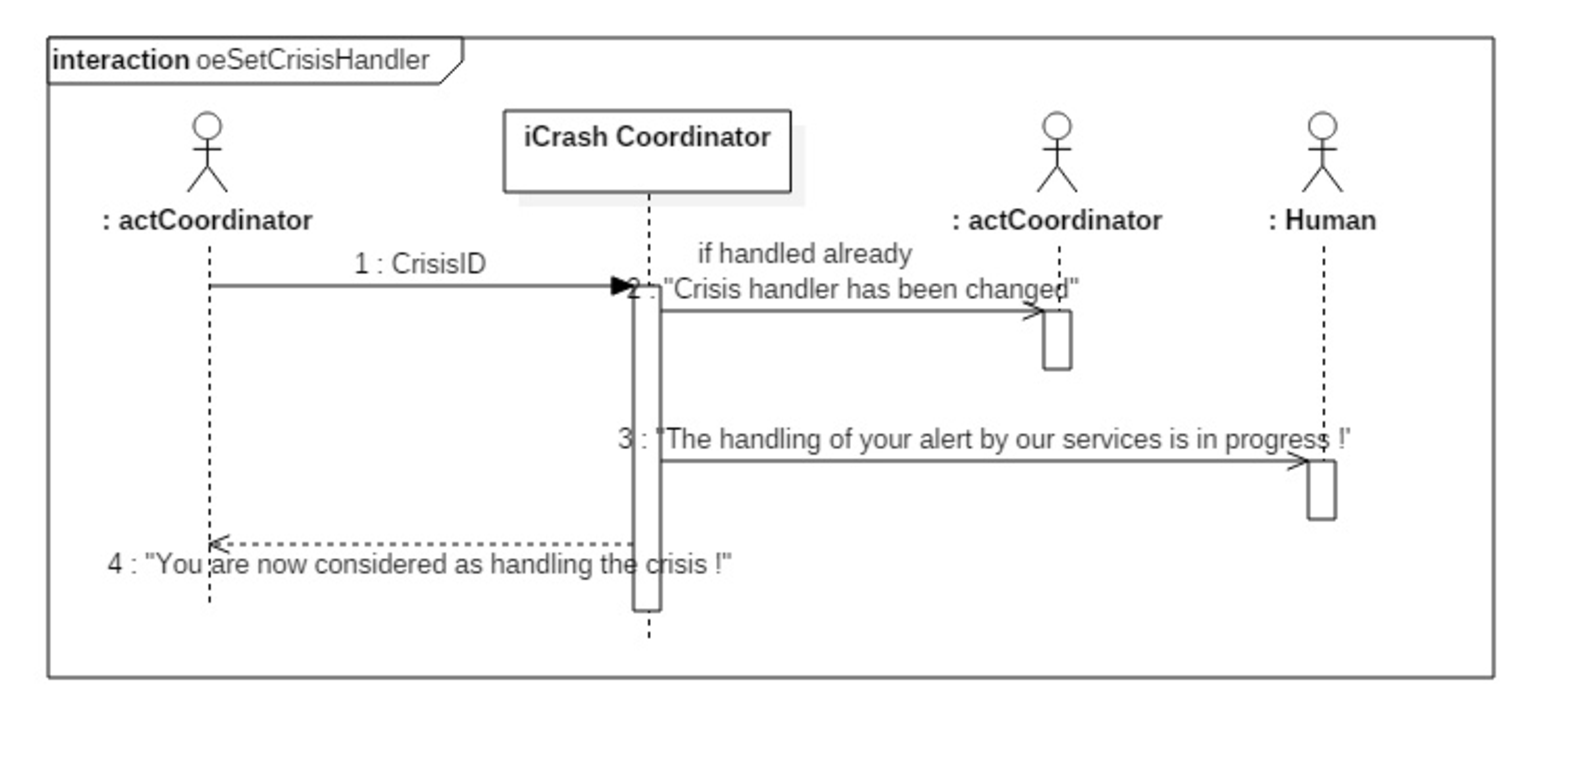
\includegraphics[width=0.5\textwidth]{./images/ui_oeSetCrisisHandler.eps}
	\caption{UI Processing view - oeSetCrisisHandler}
\end{figure}


\subsection{UI Processing view for system operation oeSetCrisisStatus}

\begin{figure}[h]
	\centering	
	\captionsetup{justification=centering}
	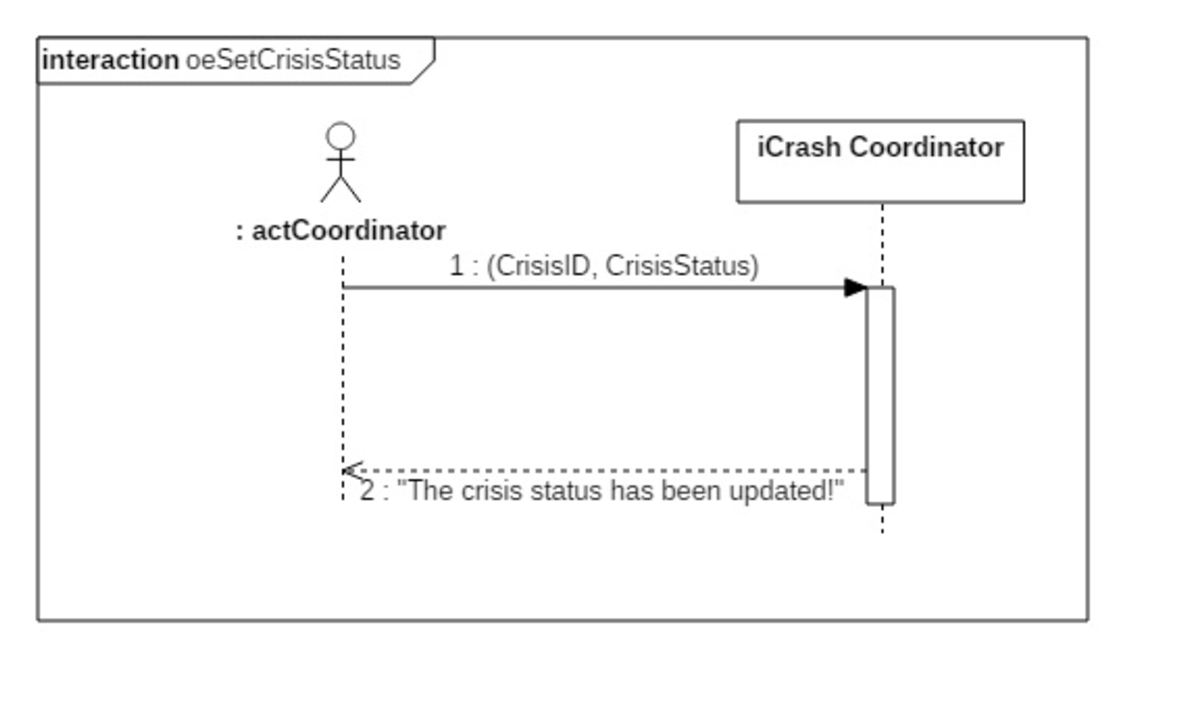
\includegraphics[width=0.5\textwidth]{./images/ui_oeSetCrisisStatus.eps}
	\caption{UI Processing view - oeSetCrisisStatus}
\end{figure}


\subsection{UI Processing view for system operation oeSetCrisisType}

\begin{figure}[h]
	\centering	
	\captionsetup{justification=centering}
	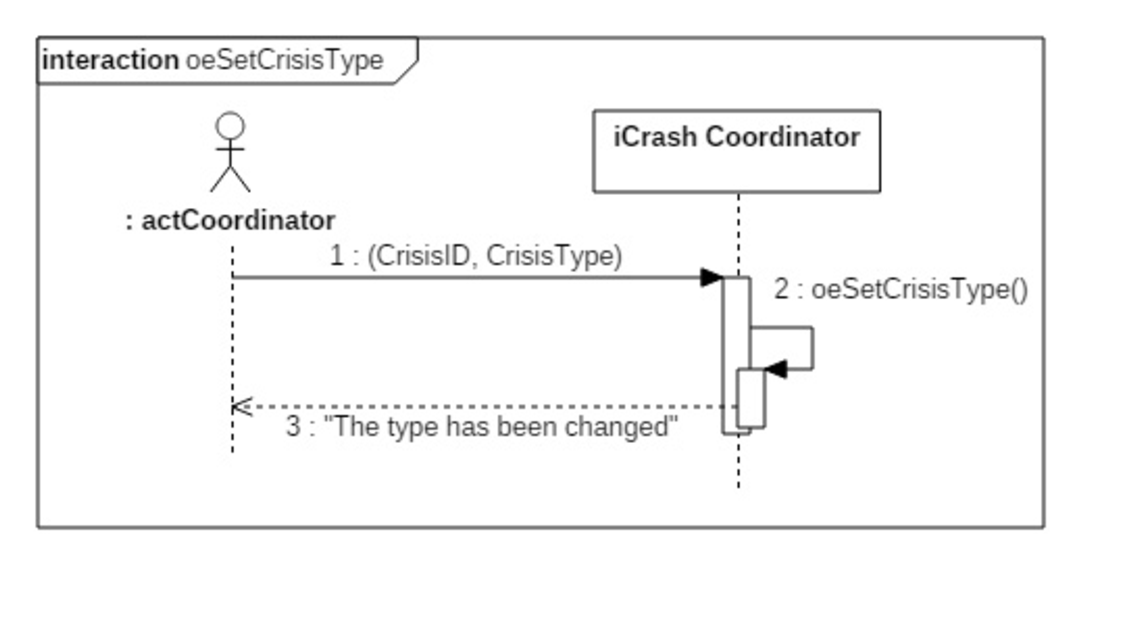
\includegraphics[width=0.5\textwidth]{./images/ui_oeSetCrisisType.eps}
	\caption{UI Processing view - oeSetCrisisType}
\end{figure}


\subsection{UI Processing view for system operation oeValidateAlert}

\begin{figure}[h]
	\centering	
	\captionsetup{justification=centering}
	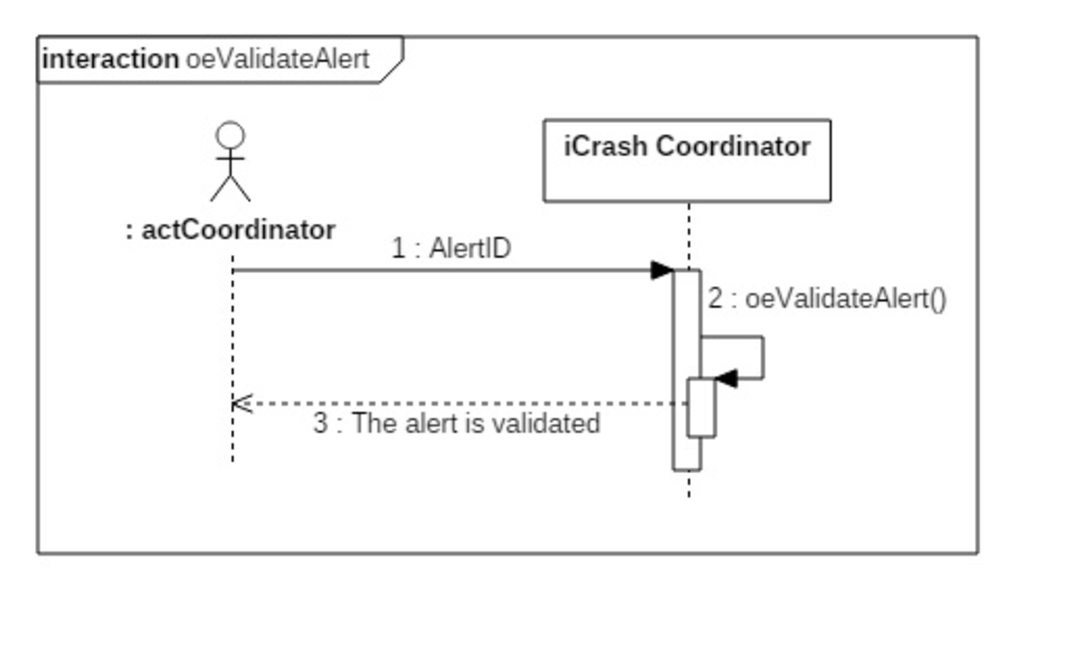
\includegraphics[width=0.5\textwidth]{./images/ui_oeValidateAlert.eps}
	\caption{UI Processing view - oeValidateAlert}
\end{figure}



\section{Non-functional runtime concerns}
The description of the runtime processes should be complemented with free
textual information regarding concurrency, distribution, performance and scalability aspects.


\subsection{Performance}
The number of incoming requests should be equal to the number of processed requests.
90 percent of response times are less than 1 sec.
CPU utilization should be below 70 percent.


\subsection{Concurrency and Parallelism}
The number of simultaneous users = the number of parallel sessions is up to 100.





\subsection{Scalability}
To support throughput increase from 1 to 10 messages per second with response
time degradation not more than 10 percent.






